\begin{figure}[h!]
\begin{center}
\centerline{\includegraphics[width=7cm]{../figures2/migration_diagram.eps}}
\caption{Migration diagram for focal player (defector on crossed site with $payoff = 1.3$). The best site in the migration range has highest payoff for the focal player (red-green site with $ = 1.3 \times 4 = 5.2$). The target site with highest payoff is occupied by a cooperative player and may be expelled with probability $s$ (orange arrow). In this case, the player on the target site is forced to move to the nearest empty site with payoff $= 2$ (black arrow pointing to light green site). However, with probability $1-s$, the focal player moves to the best empty site with payoff $=2.6$ (blue arrow pointing to light green site).}
\label{fig:migration_diagram}
\end{center}
\end{figure}


%\begin{figure}[h]
%\begin{center}
%\centerline{\includegraphics[width=18cm]{../figures2/heatmaps.eps}}
%\caption{Cooperation levels after $N=200$ iterations [i.e., $200 \times 49^2 = 480,200$ Monte Carlo Steps (MCS)] for migration Moore's distances $M = \{1,2,3,5,7,9,11,15,20 \}$, as a function of population density $d$ and probability of property violation $s$. At initialization ($t=0$), there is a $50\%$ chance that a player will cooperate (resp. defect). The uneven landscapes reflect the statistical fluctuations of simulations. For all values of $M$, the cooperation exhibits a sharp drop for $d > d^*$  and $s > s^*$ with $(d^*,s^*)$ being a function of $M$. For high grid density ($d > 0.9$), cooperation cannot be sustained even with low property violation. As the migration range gets large $M > 9$ , the area of sustainable cooperation shrinks drastically.%(see SI Section \ref{SI:d09} for further details on {\it migration} and {\it property} games in densely populated worlds).
%}
%\label{fig:heatmaps}
%\end{center}
%\end{figure}


\begin{figure}[h]
\begin{center}
\centerline{\includegraphics[width=16cm]{../figures2/phase_transition_d05.eps}}
\caption{{\bf a.} Phase transition of cooperation levels for migration Moore's distances $M = \{1,3,5,7,11\}$ and population density $d=0.5$. For all migration ranges, a tiny level of property violation $s < 0.5\%$ enhances cooperation, while more property violation decreases cooperation . For $M=1$, cooperation decreases continuously as property violation grows (up to  $s = 2\%$), For larger migration ranges, cooperation exhibits a linear decrease (given by $c = 1 ? 2.2 ? s$) up to a critical phase transition point $s^*$. As $M$ increases, $s^{*}$ becomes a range of values (color areas show the $1^{st}$ to $99^{th}$ confidence intervals), where cooperation can either be sustained at high level ($c > 0.8$), or collapse as result of a chaotic process: In this phase transition region, striving cooperation or collapse is independent of initial grid configuration. For instance, the critical phase transition range for $M=5$ (magenta area) is $ 3.7\% < s^{*} < 4.2\%$. While the outcome can either be high cooperation level or collapse, the probability of high cooperation decreases within each range critical phase transition range (c.f., continuous lines within areas): Hence, it becomes more likely that cooperation will collapse as property violation reaches the upper band of the critical phase transition range. {\bf [it's unclear why this probability is not decreasing in a monotonic way for $M=11$. It's probably a detail, but I think it's a genuine behavior that we may choose to study later on]} {\bf b.} Phase transition areas as a function of population density: For each migration range represented by color areas, the lower (dashed) boundary shows the limit below which cooperation strives systematically ($c > 0.8$), while the upper (dash-dotted) boundary shows the limit beyond which cooperation collapses systematically.  Larger migration ranges increase significantly the resistance to higher levels of property violation. However, the beneficial effects of long-range mobility are reduced for more densely populated worlds. Short range mobility ($M=1$) is highly sensitive to property violation, regardless of population density.}
\label{fig:phase_transition}
\end{center}
\end{figure}



\begin{figure}[h]
\begin{center}
\centerline{\includegraphics[width=15cm]{../figures2/tseries_transition_3.eps}}
\caption{Evolution of expected payoff increases from player rules -- success-driven migration (green), property violation (blue) or strategy update (red). expected payoff increases exhibit very similar dynamics at first ($t< 10^5$ iterations) between striving cooperation ({\bf a}) and collapse ({\bf b}) (same initial conditions: $d=0.5$,$M=5$, $s = 0.037$; colored areas show the 25\% - 75\% percentile ranges of values). At $t \approx 10^5$ iterations, structural changes occur, which decide the faith of the strive or collapse outcome: Although cooperation continues to increase until $t \approx 5\times 10^5$, in the non-sustainable case ({\bf b}) strategy update (red) yields to the highest expected payoff, while in the sustained cooperation case ({\bf a}), strategy update never provides the highest expected payoff. In the latter case, a subtle crossing occurs at the transition point  $t \approx 10^5$, where  migration transitions from the rule with the highest payoff to the lower payoff, while property violation become the rule with the highest expected payoff. The insets {\bf 1} and {\bf 2} show the correlograms between expected payoffs from the allowed actions after the tipping point: In the sustainable case ({\bf a}) cross-dependence with lag between allowed actions is very low, suggesting a strong decoupling between expected payoffs from different actions. However, in the collapsing scenario, cross-dependence remains high. Moreover, increased migration causes  more property violation (green correlogram) and more strategy updates (red correlogram). In the unsustainable scenario, cooperation still increases long after the tipping point (until $t \approx 5\times10^{5}$) and then abruptly collapses. Considering the expected mobility distance from success-driven migration (green), property violation (blue) and force move (cyan), in the collapsing scenario ({\bf d}), the expected mobility decreases but reaches quickly a high plateau ($log_{10}~U_{mobility} \approx 2.5$), while for striving societies ({\bf c}), expected mobility gets close yet higher ($1.5 < log_{10}~U_{mobility} < 2$) than the expected mobility of  property violators ($log_{10}~U_{expel} \approx 1.5$). The simulations presented here for $d=0.5$ and $M=5$ reflect the dynamics underlying the phase transitions occurring for any game with $M>1$ and for any density $0.2 \leqslant d \leqslant 0.8$.}
\label{fig:tseries}
\end{center}
\end{figure}

%\begin{figure}[h]
%\begin{center}
%%\centerline{\includegraphics[width=9cm]{../figures2/migration_transition_d05.eps}}
%\caption{Make nice grid visualizations showing (i) the tipping point and (ii) before and after the edge of collapse, and (iii) an illustration for the decoupling.}
%\label{fig:viz}
%\end{center}
%\end{figure}

\begin{figure}[h]
\begin{center}
\centerline{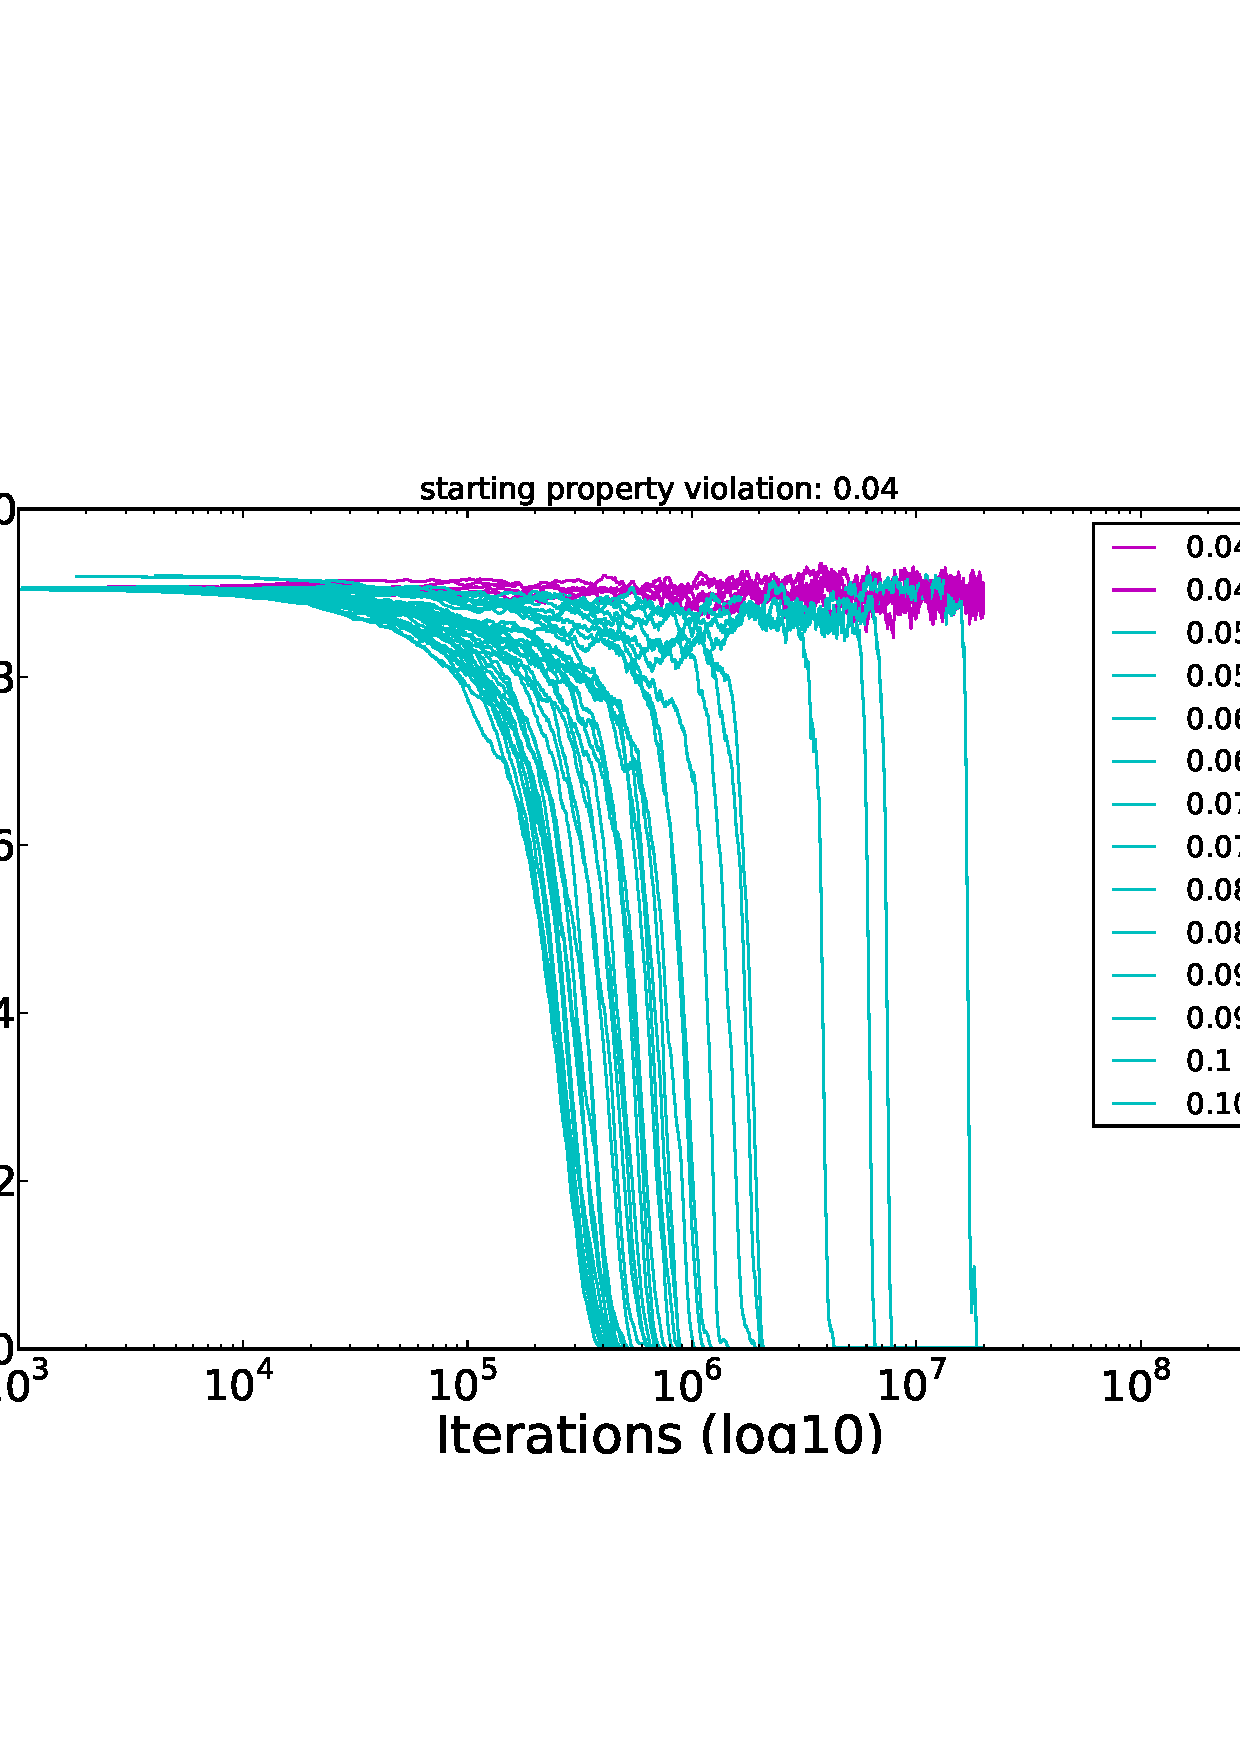
\includegraphics[width=11cm]{../figures2/resistance004.png}}
\caption{Evolution of cooperation when property violation is increased, starting from a simulation stabilized at high cooperation level ($c > 0.8$) and property violation in the upper range of the phase transition range ($s=0.040$). For $s < 0.045$ cooperation remains high, yet for  $0.05 \leqslant s \leqslant 0.06$ cooperation may collapse suddenly after $3\times10^6$ iterations (actually, it may well be that any property violation value above the phase transition region (i.e., $s=0.042$) triggers collapse after enough time, yet this collapse may be sudden and unpredictable). For $s>0.06$, the cooperation curves decreases in a more or less parabolic shape, which seems to be invariant in the limit of $s \rightarrow \infty$, and it looks like that the zero-cooperation level can be hit at earliest around $3 \times 10^5$ after the increase of property violation. {\bf [This is somehow a good news as for large increase of property violation, a rather clear downward trend appears and enough time is given to take corrective actions.]}}
\label{fig:resistance}
\end{center}
\end{figure}

\begin{figure}[h]
\begin{center}
\centerline{\includegraphics[width=15cm]{../figures2/adaptation.png}}
\caption{Temporal effects on cooperation of property violation mitigation by reducing $s$. Considering the limit case ($s = 4.2\%$) where cooperation is known to collapse after some time (black line), a  corrective action is taken to reduce property violation at a given time represented here by vertical bars. Panels {\bf a}, {\bf b}, {\bf c}, {\bf d} show the cooperation trajectories for property reduction of $10,20,50,75$ percent. Successful trajectories are shown in cyan (high level of cooperation achieved) and failed trajectories are shown in magenta (no cooperator left). Vertical bars show when the corrective action is taken (starting after $13,000$ iterations over a total of $20$ million iterations, iterations on the x-axis are presented in logarithmic scale). In general, the earlier the reduction of crime is achieved, the more likely cooperation will strive and stabilize at high levels ($c > 0.8$). However, small crime reduction of the order of 10\% ({\bf a}) hardly guaranties that a cooperative society will strive; Medium crime reduction of the order of 25\% ({\bf b}) must be taken as cooperation is still increasing; And high crime reduction [i.e. 50\% ({\bf c})] is necessary to get out the edge of collapse and further ensure and stabilize society at high cooperation levels. Only drastic crime reduction $\geqslant 75\%$ ensures restoration of cooperation at any point in time ({\bf d}). Annihilating property crime ($s=0$) helps stabilize cooperation, but at the same time removes the necessary mobility noise -- induced by small levels of property violation -- to strive (not shown).}
\label{fig:adaptation}
\end{center}
\end{figure}




%\begin{figure}[h]
%\begin{center}
%\centerline{\includegraphics[width=11cm]{../figures2/rankCrossCorr.eps}}
%\caption{Coupling / De-Coupling}
%\label{fig:crossRankCorr}
%\end{center}
%\end{figure}


%\begin{figure}[h]
%\begin{center}
%\centerline{\includegraphics[width=11cm]{../figures/configurations_t200.eps}}
%\caption{Grid configurations at $t=200$, with fully rational agents (probability of imitation $m=1$), and grid density $d=0.5$. When no migration (and {\it a fortiori} no property violation) is present (see {\it A.}), clusters of cooperators can only form by local influence, and the simulation is quickly frozen. As the migration range increases,  larger clusters form when cooperators (see {\it B.,E.}) or defectors (see {\it D.,G.}) win. At the lower limit of the phase transition point $s \rightarrow s^{*}_{-}$, cooperators form clusters, which stay strong (large?) enough to keep defectors at bay (see {\it C.,F.}).}\label{fig:comparison_no_with_migration}
%\end{center}
%\end{figure}




%\begin{figure}[h]
%\begin{center}
%\centerline{\includegraphics[width=15cm]{../figures/phase_transitions_2.eps}}
%\caption{Typical phase transitions for migration ranges $1 \leqslant M \leqslant 24$ ($0.4 \leqslant d < 0.6$). When there is no property violation $s = 0$, cooperators invade the world for any migration range $M > 0$. For small $M = \{ 1,3,5\}$, a sharp phase transition occurs at a transition point $s^{*}$, from a high level of cooperators in the populations ($c > 0.6$) when $s < s^{*}$ to entire collapse of cooperators for $s > s^{*}$. For $M \leqslant 5$, there is no intermediary state, whereas for $M \geqslant 7$, an intermediary state appears defined by $s^{*}_{-} < s < s^{*}_{+}$, with populations of cooperators in minority ($c \approx 0.45 < 0.5$) compared to defectors. For $M= \{ 7,9\}$, there is a non-zero probability of cooperation collapse, while for larger migration ranges ($M \geqslant 11$), this intermediary state becomes more stable, i.e., process converges almost surely  {\bf [to be further checked]}. Larger migration ranges increase both the maximum number of cooperators when $0 < s < s^{*}_{-}$, increase the lower $s^{*}_{-}$ and higher $s^{*}_{+}$ bounds of property violations, below (resp. above) which cooperative populations win (resp. disappear), and decreases the minimum average proportion of cooperative populations needed in order for cooperation to strive {\bf [to be further checked]}.}
%\label{fig:phase_transition}
%\end{center}
%\end{figure}








%
%
%\begin{figure}[h]
%\begin{center}
%%\centerline{\includegraphics[width=12cm]{Figures/CCDF_A.eps}}
%\caption{Representative spatial organizations for the {\it property game}: {\bf a.} Cooperation can be maintained despite 20\% of property violation probability $(M,d,s) = (9,0.5,0.2)$, {\bf b.} Cooperation collapses quickly for $s>s^*$  $(M,d,s) = (5,0.5,0.5)$, {\bf c.} and {\bf d.} phase transition at $s^{*} = 0.155\pm0.5$ and cooperation can be maintained or on the contrary collapse {\bf [discuss how it may be only a question of time before collapse $\rightarrow$ further simulations + stochastic considerations?]}, {\bf e.} Considerations for $(M,d,s) = (1, 0^+,0.5)$ (c.f. upper left panel Figure \ref{fig:cooperation_M}), and {\bf f.} Considerations for $(M,d,s) = (7,0.9,0^+)$.}
%\label{fig:configurations}
%\end{center}
%\end{figure}

